\section{Realisation}
\subsection{Engineering work}
\subsubsection{Implementation of the algorithms}
The algorithms are most of the time very straightforward.


\begin{algorithm}
 \SetAlgoLined
 \KwData{A signal spectrum X, a noise estimation Z}
 \KwResult{A new signal X' with less noise}

 \ForAll{bands $i$ in the spectrum}{
	$ t_0\gets \power(X_i)$ \\
	$ t_1 \gets t0 - \alpha * Z(i)$ \\
	$ t_2 \gets \beta * t0$ \\
	$ \mathrm{mag} \gets \sqrt{\max(t1, t2)}$ \\
	$ \mathrm{ph} \gets \phase(X_i)$ \\
	$ X_i \gets \recompute(mag, ph)$ 
	\tcp{Spectrum is given in complex format}
 }
 \caption{Simple spectral subtraction}
\end{algorithm}

\paragraph{Technologies used}
stuff
\paragraph{First organisation}
stuff
\paragraph{Mid-internship reorganisation}
\begin{figure}[H]
\begin{center}
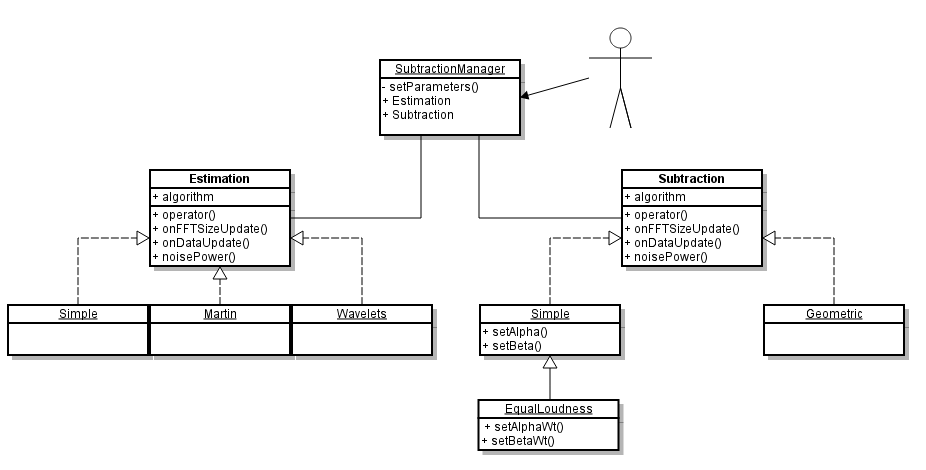
\includegraphics[scale=0.5]{diagclass.png}
\caption{Basic organization of the library}
\label{diag_api_chords}
\end{center}
\end{figure}
%Insert class diagram heres

\subsubsection{Easy way to compare algorithms}
stuff
\paragraph{Technologies used}
stuff
\subsubsection{Implementation of an English acoustic and language model}
\paragraph{Technologies used}
stuff
\subsubsection{Evaluation}
\paragraph{Signal-level evaluation}
stuff
\paragraph{Word-level evaluation}
stuff
\subsubsection{Making the processed signal listenable}
\subsection{Research work}
\subsubsection{First idea to improve spectral subtraction}
\paragraph{Kansai joint conference}
stuff
\paragraph{Evaluation}
stuff
\subsubsection{Second idea to improve spectral subtraction}
\paragraph{Evaluation}